% Chapter Template

\chapter{Design} % Main chapter title

\label{Chapter3} % Change X to a consecutive number; for referencing this chapter elsewhere, use \ref{ChapterX}

%----------------------------------------------------------------------------------------
%	SECTION 1
%----------------------------------------------------------------------------------------

\section{Conceptual overview of the system}
The system is developed as a part of the classic architectural pattern, Model-View-Controller (MVC).\color{red} (find kilde, evt. wiki) \color{black} The system itself consists of the Model and Controller part, and lets the client be responsible for the view. In figure \ref{fig:MVC} it is shown how the system is layered. As mentioned, the client is responsible of the view, which in this case is the webshop. Data is sent to the API (Controller) which simply communicates the data to the logic (model) of the system. The logic (model) is responsible for communication with the database, calculations regarding product recommendations, and handling of new incoming data.

\begin{figure}
	\centering
	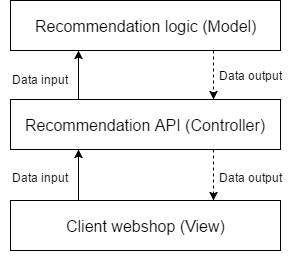
\includegraphics[width=.4\linewidth]{Figures/MVC.png}
	\caption{The Model-View-Controller (MVC) pattern applied on the system}
	\label{fig:MVC}
\end{figure}

\subsection{Recommendation API (Controller)}
The API is split into two Controller-classes, DataController and RecommendationController. If we take a look at figure \ref{fig:ControllerClasses}, the two controller-classes can be seen. The RecommendationController only consists of one API-call, however this is probably the most interesting call that can be made. Calling the GetRecommendationForVisitor-method with a visitor UID and the desired number of product recommendations will return a String-array consisting of product IDs, which the client can then use to present products in a desirable way to the end-user.\\
The DataController is used for keeping the data in the database up-to-date. The three Put-methods allows the client to provide new visitor and behavior data to the database. The GetUpdate allow the client to initiate the build of the collaborative filter. Collaborative filtering will be discussed more thoroughly in \ref{Chapters/Chapter5_Implementation}. GetUpdateVisitorTopProducts() allows the client to initiate the calculations of each visitors most viewed products. At last, CalculateTop20() lets the client initiate the calculations of the most popular products in the last 30 days. All the update-methods is special administrator methods, and should only be accessible to few access-approved staff.

\begin{figure}
	\centering
	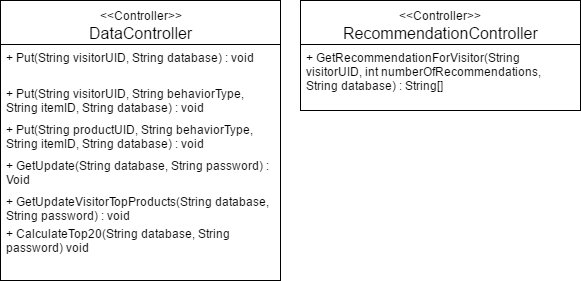
\includegraphics[width=.6\linewidth]{Figures/ControllerClasses.png}
	\caption{The two controller-classes in the recommendation API.}
	\label{fig:ControllerClasses}
\end{figure}

\subsection{Recommendation logic (Model)}
The recommendation logic is where the main operations of the system takes place. The model layer consists of five packages, and is made accessible to the controller layer through three interfaces. A package diagram of the layer can be seen in figure \ref{fig:PackageDiagram}. All classes used for calculations are placed in the Business package. This is where the product recommendations are calculated before being sent back to the control layer. This is also the package where any offline-calculation is made before it is stored in the database. The persistence package handles all information that needs to be communicated with the database. The Entities and Utility package creates an easier and more manageable way of communicating data around within the model layer. All communication between the Controller-layer and the Model-layer is done through the interfaces seen in the Communication package. These interfaces are implemented by their corresponding classes in the Business and Persistence packages. The implementation of the Model-layer is discussed further in the \ref{Chapters/Chapter5_Implementation}.

\begin{figure}
	\centering
	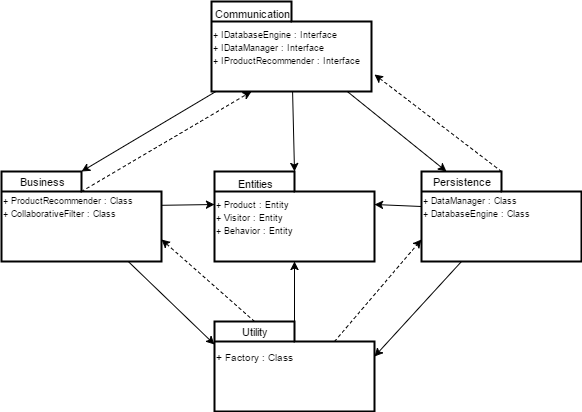
\includegraphics[width=.8\linewidth]{Figures/PackageDiagram.png}
	\caption{Package diagram of the model layer}
	\label{fig:PackageDiagram}
\end{figure}

\section{Client-Server}
When put to use, the recommendation system will be distributed and play the server role in a Client-Server model. The system should be considered an application solely for providing product recommendations. This means we have a very thin client, as its only job is to ask for recommendations by sending very little information. In this scenario, the client is the webshop that needs to provide recommendations to one of its users. The client is also able to ask the server to update its database or store new content in the database, but the concept is the same and just as simple as the request for product recommendations. The Client-Server model of the system can be seen in figure \ref{fig:ClientServer}

\begin{figure}
	\centering
	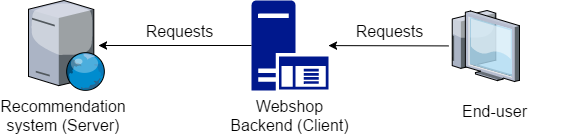
\includegraphics[width=.8\linewidth]{Figures/ClientServer.png}
	\caption{Package diagram of the model layer}
	\label{fig:ClientServer}
\end{figure}

\section{Database design}
One of the challenges of the project was to come up with a database design that would meet the requirements of the final product.